\documentclass{article}
\usepackage[margin=0.5in,vmargin=0.5in]{geometry}
\usepackage{tikz}
\usepackage{graphicx}

%% neural network parameters
\newcommand\widthCirc{.5} % size of all circles
\newcommand\otdis{3} % distance between layers
\newcommand\nodeSep{2} % node seperation along y axis
\newcommand\inputNodes{2} % input node count
\newcommand\hiddenNodes{3} % hidden node count
\newcommand\outputNodes{1} % output node count
\newcommand\inputSRow{1} % vertical off-set of input layer
\newcommand\hiddenSRow{0} % vertical off-set of hidden layer
\newcommand\outputSRow{2} % vertical off-set of output layer
\newcommand\numLayers{3} % number of layers ommiting output layer


\newcommand\twohiddenNodes{2} % second hidden layer node count
\newcommand\twohiddenSRow{1} % vertical off-set of second hidden layer

\newcommand\wpadding{0.25} % width padding for layer box
\newcommand\hpadding{0.75} % height padding for layer box
\newcommand\ytilt{0.25} % tilt for effect

\begin{document}

\begin{centering}

  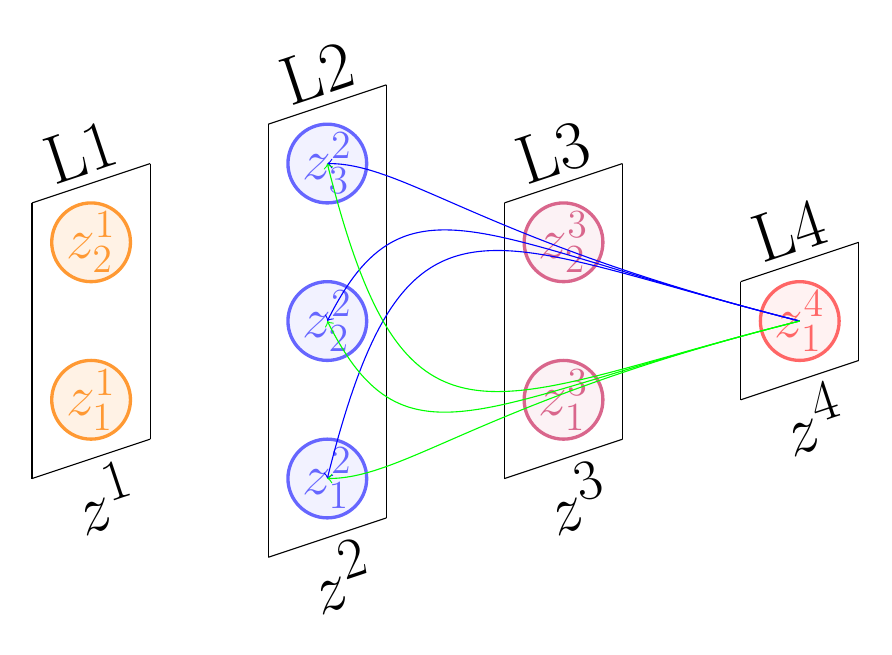
\begin{tikzpicture}
    \foreach \Rnumber in {1,...,\inputNodes}{
      \filldraw[color=orange!80, fill=orange!10, very thick](0,\inputSRow+\nodeSep*\Rnumber) circle (\widthCirc) node {\huge{$z^{1}_{\Rnumber}$}};
    }
    
    \foreach \Rnumber in {1,...,\hiddenNodes}{
      \filldraw[color=blue!60, fill=blue!5, very thick](\numLayers*\otdis-2*\otdis,\hiddenSRow+\nodeSep*\Rnumber) circle (\widthCirc) node {\huge{$z^{2}_{\Rnumber}$}};
    }

    \foreach \Rnumber in {1,...,\twohiddenNodes}{
      \filldraw[color=purple!60, fill=purple!5, very thick](\numLayers*\otdis-1*\otdis,\twohiddenSRow+\nodeSep*\Rnumber) circle (\widthCirc) node {\huge{$z^{3}_{\Rnumber}$}};
    }
    
    \foreach \Rnumber in {1,...,\outputNodes}{
      \filldraw[color=red!60, fill=red!5, very thick](\numLayers*\otdis,\outputSRow+\nodeSep*\Rnumber) circle (\widthCirc) node {\huge{$z^{4}_{\Rnumber}$}};
    }

    % drawing the boxes around the layers
 
    % LAYER ONE
    \draw[thin,black] (-\widthCirc-\wpadding,\inputSRow+\nodeSep-\hpadding-\ytilt) -- (-\widthCirc-\wpadding,\inputSRow+\nodeSep*\inputNodes+\hpadding-\ytilt) {};
    \draw[thin,black] (\widthCirc+\wpadding,\inputSRow+\nodeSep-\hpadding+\ytilt) -- (\widthCirc+\wpadding,\inputSRow+\nodeSep*\inputNodes+\hpadding+\ytilt) {};
    \draw[thin,black] (-\widthCirc-\wpadding,\inputSRow+\nodeSep*\inputNodes+\hpadding-\ytilt) -- (\widthCirc+\wpadding,\inputSRow+\nodeSep*\inputNodes+\hpadding+\ytilt) node [midway, above, sloped] (TextNode) {\Huge{L1}};
    \draw[thin,black] (-\widthCirc-\wpadding,\inputSRow+\nodeSep-\hpadding-\ytilt) -- (\widthCirc+\wpadding,\inputSRow+\nodeSep-\hpadding+\ytilt) node [midway, below, sloped] (TextNode) {\Huge{$z^{1}$}}; 

    % LAYER TWO
    \draw[thin,black] (\otdis-\widthCirc-\wpadding,\hiddenSRow+\nodeSep-\hpadding-\ytilt) -- (\otdis-\widthCirc-\wpadding,\hiddenSRow+\nodeSep*\hiddenNodes+\hpadding-\ytilt) {};
    \draw[thin,black] (\otdis+\widthCirc+\wpadding,\hiddenSRow+\nodeSep-\hpadding+\ytilt) -- (\otdis+\widthCirc+\wpadding,\hiddenSRow+\nodeSep*\hiddenNodes+\hpadding+\ytilt) {};
    \draw[thin,black] (\otdis-\widthCirc-\wpadding,\hiddenSRow+\nodeSep*\hiddenNodes+\hpadding-\ytilt) -- (\otdis+\widthCirc+\wpadding,\hiddenSRow+\nodeSep*\hiddenNodes+\hpadding+\ytilt) node [midway, above, sloped] (TextNode) {\Huge{L2}};
    \draw[thin,black] (\otdis-\widthCirc-\wpadding,\hiddenSRow+\nodeSep-\hpadding-\ytilt) -- (\otdis+\widthCirc+\wpadding,\hiddenSRow+\nodeSep-\hpadding+\ytilt) node [midway, below, sloped] (TextNode) {\Huge{$z^{2}$}};

    % LAYER THREE
    \draw[thin,black] (\otdis+\otdis-\widthCirc-\wpadding,\twohiddenSRow+\nodeSep-\hpadding-\ytilt) -- (\otdis+\otdis-\widthCirc-\wpadding,\twohiddenSRow+\nodeSep*\twohiddenNodes+\hpadding-\ytilt) {};
    \draw[thin,black] (\otdis+\otdis+\widthCirc+\wpadding,\twohiddenSRow+\nodeSep-\hpadding+\ytilt) -- (\otdis+\otdis+\widthCirc+\wpadding,\twohiddenSRow+\nodeSep*\twohiddenNodes+\hpadding+\ytilt) {};
    \draw[thin,black] (\otdis+\otdis-\widthCirc-\wpadding,\twohiddenSRow+\nodeSep*\twohiddenNodes+\hpadding-\ytilt) -- (\otdis+\otdis+\widthCirc+\wpadding,\twohiddenSRow+\nodeSep*\twohiddenNodes+\hpadding+\ytilt) node [midway, above, sloped] (TextNode) {\Huge{L3}};
    \draw[thin,black] (\otdis+\otdis-\widthCirc-\wpadding,\twohiddenSRow+\nodeSep-\hpadding-\ytilt) -- (\otdis+\otdis+\widthCirc+\wpadding,\twohiddenSRow+\nodeSep-\hpadding+\ytilt) node [midway, below, sloped] (TextNode) {\Huge{$z^{3}$}};

    % LAYER FOUR
    \draw[thin,black] (\otdis+\otdis+\otdis-\widthCirc-\wpadding,\outputSRow+\nodeSep-\hpadding-\ytilt) -- (\otdis+\otdis+\otdis-\widthCirc-\wpadding,\outputSRow+\nodeSep*\outputNodes+\hpadding-\ytilt) {};
    \draw[thin,black] (\otdis+\otdis+\otdis+\widthCirc+\wpadding,\outputSRow+\nodeSep-\hpadding+\ytilt) -- (\otdis+\otdis+\otdis+\widthCirc+\wpadding,\outputSRow+\nodeSep*\outputNodes+\hpadding+\ytilt) {};
    \draw[thin,black] (\otdis+\otdis+\otdis-\widthCirc-\wpadding,\outputSRow+\nodeSep*\outputNodes+\hpadding-\ytilt) -- (\otdis+\otdis+\otdis+\widthCirc+\wpadding,\outputSRow+\nodeSep*\outputNodes+\hpadding+\ytilt)  node [midway, above, sloped] (TextNode) {\Huge{L4}};
    \draw[thin,black] (\otdis+\otdis+\otdis-\widthCirc-\wpadding,\outputSRow+\nodeSep-\hpadding-\ytilt) -- (\otdis+\otdis+\otdis+\widthCirc+\wpadding,\outputSRow+\nodeSep-\hpadding+\ytilt) node [midway, below, sloped] (TextNode) {\Huge{$z^{4}$}};

    % PATHS OF MANY ERROR

    % error from z^{3}_{2}
    \draw [blue,thin,->] (\numLayers*\otdis,\outputSRow+\nodeSep) .. controls (\otdis+\otdis-1,\twohiddenSRow+\nodeSep*2) and (\otdis+\otdis-2,\twohiddenSRow+\nodeSep*2+1) .. (\otdis,\hiddenSRow+\nodeSep*3);
    \draw [blue,thin,->] (\numLayers*\otdis,\outputSRow+\nodeSep) .. controls (\otdis+\otdis-1,\twohiddenSRow+\nodeSep*2) and (\otdis+\otdis-2,\twohiddenSRow+\nodeSep*2+1) .. (\otdis,\hiddenSRow+\nodeSep*2);
    \draw [blue,thin,->] (\numLayers*\otdis,\outputSRow+\nodeSep) .. controls (\otdis+\otdis-1,\twohiddenSRow+\nodeSep*2) and (\otdis+\otdis-2,\twohiddenSRow+\nodeSep*2+1) .. (\otdis,\hiddenSRow+\nodeSep*1);

    % error from z^{3}_{1}
    \draw [green,thin,->] (\numLayers*\otdis,\outputSRow+\nodeSep) .. controls (\otdis+\otdis-1,\twohiddenSRow+\nodeSep*1) and (\otdis+\otdis-2,\twohiddenSRow+\nodeSep*1-1) .. (\otdis,\hiddenSRow+\nodeSep*3);
    \draw [green,thin,->] (\numLayers*\otdis,\outputSRow+\nodeSep) .. controls (\otdis+\otdis-1,\twohiddenSRow+\nodeSep*1) and (\otdis+\otdis-2,\twohiddenSRow+\nodeSep*1-1) .. (\otdis,\hiddenSRow+\nodeSep*2);
    \draw [green,thin,->] (\numLayers*\otdis,\outputSRow+\nodeSep) .. controls (\otdis+\otdis-1,\twohiddenSRow+\nodeSep*1) and (\otdis+\otdis-2,\twohiddenSRow+\nodeSep*1-1) .. (\otdis,\hiddenSRow+\nodeSep*1);

  \end{tikzpicture}
\end{centering}

\end{document}
